\documentclass{standalone}
\usepackage{tikz}
\usepackage{pgfplots}

\tikzset{align at bottom/.style={baseline=(current bounding box.south)}}

\begin{document} 
	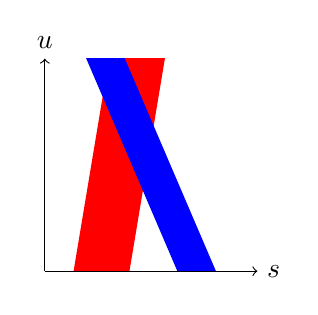
\begin{tikzpicture}[scale = 0.27]
	
		\begin{scope}
			\clip (-5, -5) rectangle (5, 5);
			\draw[scale = 1, smooth, variable = \x, red, line width = 0.7cm] plot ({\x}, { 12 / 2 * (\x + 1.5)});
			\draw[scale = 1, smooth, variable = \x, blue, line width = 0.45cm] plot ({\x}, { -7 / 3 * \x});
		\end{scope}
		
		\draw[->] (-5, -5) -- (5, -5) node[right] {$s$};
		\draw[->] (-5, -5) -- (-5, 5) node[above] {$u$};
		
	\end{tikzpicture}
\end{document}